\documentclass[10pt]{article}
\usepackage{fullpage}
\usepackage{amsmath}
\usepackage{mathtools}
\usepackage{setspace}
\usepackage{float}
\doublespacing

\begin{document}

\title{Homework 3}
\date{}

\maketitle

\section{Decision Tree}

\subsection{Problem 1}

A decision tree can separate those points correctly. We can construct this decision tree as follows. For any point $(x_{i1}, x_{i2})$. First look at the first feature $x_{i1}$. Find the interval it falls into and then do a corresponding split according to the second feature $x_{i2}$. The figure \ref{fig1} gives an intuitive explanation. The depth of the decision tree depth on the way of constructing. We can construct a tree with depth 2. The first part has N branches and it does a split according to the value on first dimension and in second part each node has 2 branches and it will split according to second dimension. If we use a binary tree to do classification the depth of the corresponding binary tree is $N$. 

\begin{figure}[H]
\centering
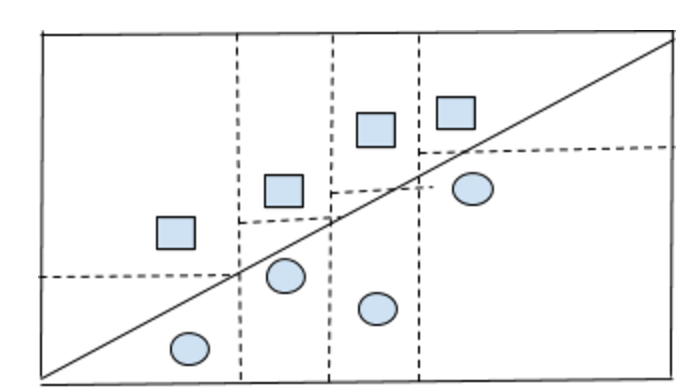
\includegraphics[width=0.5\textwidth]{fig1.png}
\caption{\label{fig1} tree of a linear classifier}
\end{figure}

\subsection{Problem 2}

Those points can be classified correctly with a decision tree. A decision tree can do any division on the feature space. The strategy is as follows. First do a split on the first dimension of $\mathbf{x}$ to get $k$ intervals and ensure in each interval there exists only one value. Suppose there exists $n_i$ different values of second dimension in $i$th interval(i.e $n_i$ points in the interval). Any labeling can be done by at most $n_i$ splits. The depth of the tree still depends on the form of the tree. If it does not have to be a binary tree, the depth is 2 with $i$th part doing a split according to feature in $i$th dimension($i=1,2$). If it should be a binary tree the depth will be equal to $p$ which is the number of distinct feature value in 1st dimension.

\section{Boosting}
\subsection{Problem 3}

Suppose the weighted error is $L(h_{T+1})$

\begin{equation}
\begin{aligned}
\begin{split}
& L(h_{t+1}) = \sum_{i=1}^{N}\frac{W_{i}^{T+1}}{Z_{T+1}}L_{0/1}(y_{i}, h_{T+1}(x_i)) \\
& = \sum_{i:y_i\neq h_{T+1}(x_i)}\frac{W_{i}^{T+1}}{Z_{T+1}} \\ 
& = \sum_{i:y_i\neq h_{T+1}(x_i)}\frac{W_{i}^{T}\cdot e^{\alpha_{T+1}}}{Z_{T+1}} \\
\end{split}
\end{aligned}
\end{equation}

As $\epsilon_{T+1}=\sum_{i:y_i\neq h_{T+1}(x_i)}W_{i}^{T}$, $\alpha_{T+1}=\frac{1}{2}log\frac{1-\epsilon_{T+1}}{\epsilon_{T+1}}$, we can calculate $Z_{T+1}$ as follows:

\begin{equation}
\begin{aligned}
\begin{split}
& Z_{T+1} = \sum_{i} W_{i}^{T+1} \\
& = \sum_{i}W_{i}^{T}\cdot e^{-\alpha_{T+1}y_{i}h_{T+1}(x_i)} \\
& = e^{-\alpha_{T+1}}(1-\epsilon_{T+1}) + e^{\alpha_{T+1}}\epsilon_{T+1} \\
& = 2\sqrt{\epsilon_{T+1}(1-\epsilon_{T+1})}
\end{split}
\end{aligned}
\end{equation}

Thus, 

\begin{equation}
\begin{aligned}
\begin{split}
& L = \frac{\epsilon_{T+1}\cdot \sqrt{\frac{1-\epsilon_{T+1}}{\epsilon_{T+1}}}}{2\sqrt{\epsilon_{T+1}(1-\epsilon_{T+1})}} \\
& = \frac{1}{2} \\
\end{split}
\end{aligned}
\end{equation}

\subsection{Problem 4}

Suppose exponential loss of $H_t$($=\sum_{i}\alpha_{i}h_i$) is $L$. Then,

\begin{equation}
\begin{aligned}
& L = \sum_{i=1}^{N}W_{i}^{t} \\
& = \sum_{i=1}^{N}W_{i}^{t-1}\cdot e^{-\alpha_{t}y_{i}h_{t}(x_i)} \\
& = \sum_{i:y_{i}\neq h_{t}(x_i)}W_{i}^{t-1}\cdot e^{\alpha_{t}} + \sum_{i:y_{i}= h_{t}(x_i)}W_{i}^{t-1}\cdot e^{-\alpha_{t}} \\
& = e^{\alpha_{t}}\cdot \epsilon_{t} + e^{-\alpha_{t}}\cdot (1- \epsilon_{t}) \\
\end{aligned}
\end{equation}

To minimize $L$, we need to set $\frac{dL}{d\alpha_t}$ to zero.

\begin{equation}
\begin{aligned}
& \frac{dL}{d\alpha_t} = 0 \\
& \implies \frac{dL}{d\alpha_t}= e^{-\alpha_t}(\epsilon_t-1)+e^{\alpha_t}\cdot \epsilon_t = 0 \\
& \implies \alpha_t= \frac{1}{2}log\frac{1-\epsilon_t}{\epsilon_t} \\
\end{aligned}
\end{equation}


\section{SVM}

This is a solution to problem in non-separable case. Its equivalent dual form is as follows.

\begin{equation}
\begin{aligned}
& max{\sum_{i=1}^{N}\alpha_{i}-\frac{1}{2}\sum_{i,j=1}^{N}\alpha_{i}\alpha_{j}y_{i}y_{j}\mathbf{x}_{i}\mathbf{x}_{j}} \\
& s.t. \sum_{i=1}^{N}\alpha_{i}y_{i} = 0, 0\leq \alpha\leq C \\
& w=\sum_{i=1}^{N}\alpha_{i}y_{i}\mathbf{x}_i \\
\end{aligned}
\end{equation}

We can set following matrices to represent it in standard form:
$\mathbf{f}=\begin{pmatrix}
-1 \\
\vdots \\
-1 \\
\end{pmatrix}$, 
$\mathbf{\alpha}=\begin{pmatrix}
\alpha_1 \\
\vdots \\
\alpha_N \\
\end{pmatrix}$, 
$\mathbf{B}=(y_1,\cdots, y_N)$,
$\mathbf{H}=\begin{pmatrix}
y_{1}y_{1}K(x_1, x_1) & \cdots & y_{1}y_{N}K(x_{1}, x_{N}) \\
\vdots & \ddots & \vdots \\
y_{N}y_{1}K(x_N, x_1) & \cdots & y_{N}y_{N}K(x_{N}, x_{N}) 
\end{pmatrix}=diag(y_1, \cdots, y_N)\mathbf{K}diag(y_1, \cdots, y_N)$,
$\mathbf{A}=\begin{pmatrix}
1 & &  \\
& \ddots & \\
 & & 1 \\
 -1 & &  \\
  & \ddots & \\
 & & -1 \\
\end{pmatrix}$,
$\mathbf{a}=\begin{pmatrix}
c \\
\vdots \\
c \\
0 \\
\vdots \\
0 \\
\end{pmatrix}$

With the above notations, we can represent the original problem in matrix form as follows.

\begin{equation}
\begin{aligned}
& argmin \frac{1}{2}\alpha^{T}\mathbf{H}\alpha + \mathbf{f}^{T}\alpha \\
& s.t. \mathbf{A}\alpha \leq \mathbf{a} \\
& \mathbf{B\alpha}=\mathbf{0} \\
\end{aligned}
\end{equation}

%--BIBLIOGRAPHY--%
% \begin{thebibliography}{99}

% \bibitem{SampleBibLabel} Author, "Title",  Journal, Volume, Pages, Year. \\
% This is the annotation for this bibliographic record.

% \end{thebibliography}

\end{document}
